\cleardoublepage



\chapter{Résultats - Discussion}

Nous avons pu terminer le projet dans les temps seulement, même si celui-ci est aujourd'hui fonctionnel, il persiste encore certains problèmes. Nous avons toujours essayer de les
résoudre de la manière la plus efficiente qui soit. Seulement, il nous est arrivé de bloquer sur des
parties pour lesquelles aucune solutions propres n'étaient réalisable. Nous avons alors du appliquer 
des manipulations qui empêcheront ce projet d'être un projet considéré comme stable dans un environnement
grand public.





%%%%%%%%%%%%%%%%%%%%%%%%%%%%%%%%%%%%%%%%%%%%%%%%%%%%%%%%%%%%%%%%%%%%%%%%%%%%%%%%%%%%%%%%%%%%%%%%%%%%
%%%%%%%%%%%%%%%%%%%%%%%%%%%%%%%%%%%%%%%%%%%%%%%%%%%%%%%%%%%%%%%%%%%%%%%%%%%%%%%%%%%%%%%%%%%%%%%%%%%%
%%%%%%%%%%%%%%%%%%%%%%%%%%%%%%%%%%%%%%%%%%%%%%%%%%%%%%%%%%%%%%%%%%%%%%%%%%%%%%%%%%%%%%%%%%%%%%%%%%%%
%%%%%%%%%%%%%%%%%%%%%%%%%%%%%%%%%%%%%%%%%%%%%%%%%%%%%%%%%%%%%%%%%%%%%%%%%%%%%%%%%%%%%%%%%%%%%%%%%%%%
%%%%%%%%%%%%%%%%%%%%%%%%%%%%%%%%%%%%%%%%%%%%%%%%%%%%%%%%%%%%%%%%%%%%%%%%%%%%%%%%%%%%%%%%%%%%%%%%%%%%

\section{Protocole de transfert}

Le choix de prendre GTalk comme moyen de communication n'était pas sans conséquences.
En effet, il nous est apparu impossible d'avoir une gestion fine de GTalk.



%%%%%%%%%%%%%%%%%%%%%%%%%%%%%%%%%%%%%%%%%%%%%%%%%%%%%%%%%%%%%%%%%%%%%%%%%%%%%%%%%%%%%%%%%%%%%%%%%%%%
%%%%%%%%%%%%%%%%%%%%%%%%%%%%%%%%%%%%%%%%%%%%%%%%%%%%%%%%%%%%%%%%%%%%%%%%%%%%%%%%%%%%%%%%%%%%%%%%%%%%
%%%%%%%%%%%%%%%%%%%%%%%%%%%%%%%%%%%%%%%%%%%%%%%%%%%%%%%%%%%%%%%%%%%%%%%%%%%%%%%%%%%%%%%%%%%%%%%%%%%%

\subsection{Réception et traitement}

Lors de l'envoi d'un message XMPP d'un compte A vers un compte B, toutes les interfaces de connexions de B recevront le message.
Alors l'envoi d'un message XMPP d'un compte A vers ce même compte A, le message sera aussitôt reçu par A.

Dans notre cas le fait d'envoyer un message XMPP sur notre propre compte revient à recevoir et traiter ce même message que l'on vient d'envoyer.
Bien heureusement nos applications filtreront les messages qui ne leur sont pas destinés.

\begin{figure}[!h]
	\center
	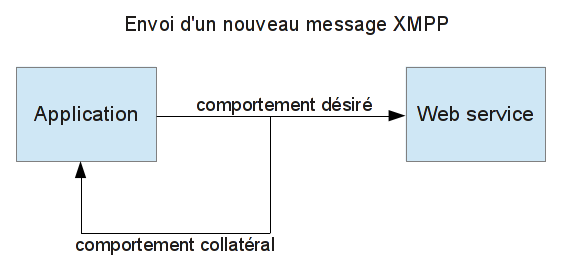
\includegraphics[width=12cm]{img/boucle-envoi-xmpp.png}
	\caption{Création d'une boucle lors de l'envoi d'un message XMPP}
	\label{boucle-envoi-xmpp}
\end{figure}

Comme le montre l'image \ref{boucle-envoi-xmpp}, une boucle se crée.
Dans les faits elle ne causera jamais de problème, néanmoins c'est un comportement qui n'était pas désiré et qu'on aurait souhaité éviter.



%%%%%%%%%%%%%%%%%%%%%%%%%%%%%%%%%%%%%%%%%%%%%%%%%%%%%%%%%%%%%%%%%%%%%%%%%%%%%%%%%%%%%%%%%%%%%%%%%%%%
%%%%%%%%%%%%%%%%%%%%%%%%%%%%%%%%%%%%%%%%%%%%%%%%%%%%%%%%%%%%%%%%%%%%%%%%%%%%%%%%%%%%%%%%%%%%%%%%%%%%
%%%%%%%%%%%%%%%%%%%%%%%%%%%%%%%%%%%%%%%%%%%%%%%%%%%%%%%%%%%%%%%%%%%%%%%%%%%%%%%%%%%%%%%%%%%%%%%%%%%%

\subsection{"Broadcast"}

Les messages XMPP ne se limitent pas aux quelques clients présents dans notre projet : site web et applications mobiles.
Tous les messages que nous envoyons sont aussi redirigés vers les outils utilisant GTalk.

En pratique, cela impliquait de recevoir des messages au format JSon sur plusieurs lieux indésirables.

\begin{figure}[!h]
	\center
	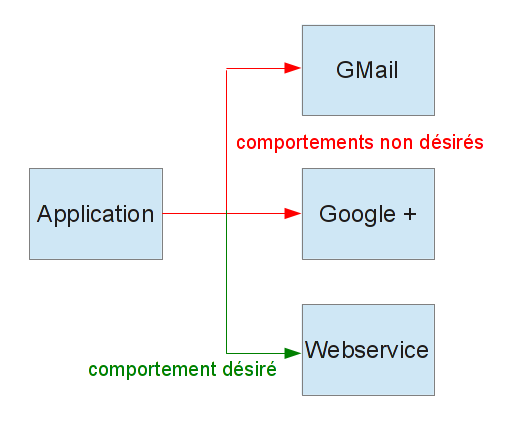
\includegraphics[width=10cm]{img/broadcast-xmpp.png}
	\caption{Destinataires lors d'un envoi d'un message XMPP}
	\label{broadcast-xmpp}
\end{figure}

Comme le montre le schéma \ref{broadcast-xmpp}, lors de l'envoi d'un message XMPP originellement destiné uniquement à une application ou au webservice, c'est tous l'environnement qui reçoit et affiche le nouveaux messages.
Le résultat est montré dans l'image \ref{message-xmpp-json-gmail}, un message XMPP au format JSON. 
	
\begin{figure}[!h]
	\center
	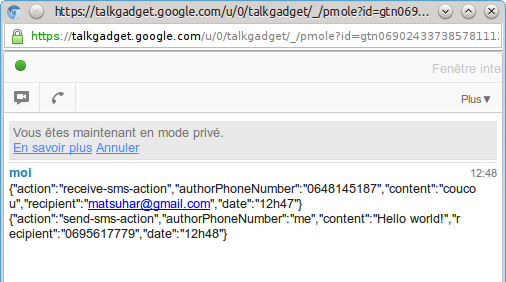
\includegraphics[width=10cm]{img/message-xmpp-json-gmail.png}
	\caption{Message XMPP au format JSON reçu avec GTalk}
	\label{message-xmpp-json-gmail}
\end{figure}





%%%%%%%%%%%%%%%%%%%%%%%%%%%%%%%%%%%%%%%%%%%%%%%%%%%%%%%%%%%%%%%%%%%%%%%%%%%%%%%%%%%%%%%%%%%%%%%%%%%%
%%%%%%%%%%%%%%%%%%%%%%%%%%%%%%%%%%%%%%%%%%%%%%%%%%%%%%%%%%%%%%%%%%%%%%%%%%%%%%%%%%%%%%%%%%%%%%%%%%%%
%%%%%%%%%%%%%%%%%%%%%%%%%%%%%%%%%%%%%%%%%%%%%%%%%%%%%%%%%%%%%%%%%%%%%%%%%%%%%%%%%%%%%%%%%%%%%%%%%%%%
%%%%%%%%%%%%%%%%%%%%%%%%%%%%%%%%%%%%%%%%%%%%%%%%%%%%%%%%%%%%%%%%%%%%%%%%%%%%%%%%%%%%%%%%%%%%%%%%%%%%
%%%%%%%%%%%%%%%%%%%%%%%%%%%%%%%%%%%%%%%%%%%%%%%%%%%%%%%%%%%%%%%%%%%%%%%%%%%%%%%%%%%%%%%%%%%%%%%%%%%%

\section{Site web}

Concernant le site web, les résultats obtenus sont probants.
Néanmoins, plusieurs fonctionnalités auxquels nous avions pensé manquent.



%%%%%%%%%%%%%%%%%%%%%%%%%%%%%%%%%%%%%%%%%%%%%%%%%%%%%%%%%%%%%%%%%%%%%%%%%%%%%%%%%%%%%%%%%%%%%%%%%%%%
%%%%%%%%%%%%%%%%%%%%%%%%%%%%%%%%%%%%%%%%%%%%%%%%%%%%%%%%%%%%%%%%%%%%%%%%%%%%%%%%%%%%%%%%%%%%%%%%%%%%
%%%%%%%%%%%%%%%%%%%%%%%%%%%%%%%%%%%%%%%%%%%%%%%%%%%%%%%%%%%%%%%%%%%%%%%%%%%%%%%%%%%%%%%%%%%%%%%%%%%%

\subsection{Gestion des contacts}

%%%%%%%%%%%%%%%%%%%%%%%%%%%%%%%%%%%%%%%%%%%%%%%%%%%%%%%%%%%%%%%%%%%%%%%%%%%%%%%%%%%%%%%%%%%%%%%%%%%%

\subsubsection{Cahier des charges}

Notre cahier des charges requérait une gestion simple et transparente des contacts pour l'utilisateur.

Le téléchargement des contacts du compte Google couplé avec l'affichage de la liste des noms de ces contacts, permet à l'utilisateur d'envoyer des SMS très simplement sans avoir à spécifier le numéro de téléphone.

%%%%%%%%%%%%%%%%%%%%%%%%%%%%%%%%%%%%%%%%%%%%%%%%%%%%%%%%%%%%%%%%%%%%%%%%%%%%%%%%%%%%%%%%%%%%%%%%%%%%

\subsubsection{Problème}

Comme expliqué dans la partie \ref{Téléchargement des contacts Google} les contacts présents sur les smartphones Androïd sont synchronisés avec le même compte Gmail.
Sous iOS cette fonction existe mais n'est pas associé à Google : Apple utilise iCloud qui permet aux utilisateurs une synchronisation automatique des contacts sur tous les appareils Apple associés à l'adresse mail.
Ainsi par défaut il n'est pas possible d'accéder aux contacts de l'iPhone depuis le site web.

Contrairement à Google qui effectue ses authentifications avec OAuth, Apple ne propose pas d'API permettant l'authentification sur iCloud.
La solution trouvée a donc été de synchroniser les contacts de l'iPhone avec un compte Google, au détriment de la synchronisation d'iCloud.

%%%%%%%%%%%%%%%%%%%%%%%%%%%%%%%%%%%%%%%%%%%%%%%%%%%%%%%%%%%%%%%%%%%%%%%%%%%%%%%%%%%%%%%%%%%%%%%%%%%%

\subsubsection{Amélioration possibles}

\Jparagraph{Filtres}

Dans notre site web nous avons filtré la liste des contacts à ceux présents dans notre carnet d'adresses et en nous limitant aux numéros de téléphone portable (06.xx.xx.xx.xx ou 07.xx.xx.xx.xx).
Or il est possible de recevoir des SMS venant de numéro "courts" (8.xx.xx), de numéros de téléphone fixe, ou bien encore de contacts non présents dans nos contacts.

Notre version actuelle ne permet pas de résoudre ce problème.
Une solution serait d'ajouter un filtre sur la page web et enregistrer tous les contacts ainsi que ceux non présents dans Google.


\Jparagraph{Anciens SMS}

Lorsque l'on se déconnecte du site web toutes les conversations sont supprimées du serveur en raison de la politique de sécurisé que nous avons voulu garder.

Nous avons pensé apporter une amélioration à notre site web dans la prochaine version, qui aurait pour objectif de télécharger les anciens messages échangés avec un contact.
Ces SMS transiteraient aussi par le protocole XMPP, soit un par un, soit sous forme de liste selon les performances et la taille maximale des messages XMPP.



%%%%%%%%%%%%%%%%%%%%%%%%%%%%%%%%%%%%%%%%%%%%%%%%%%%%%%%%%%%%%%%%%%%%%%%%%%%%%%%%%%%%%%%%%%%%%%%%%%%%
%%%%%%%%%%%%%%%%%%%%%%%%%%%%%%%%%%%%%%%%%%%%%%%%%%%%%%%%%%%%%%%%%%%%%%%%%%%%%%%%%%%%%%%%%%%%%%%%%%%%
%%%%%%%%%%%%%%%%%%%%%%%%%%%%%%%%%%%%%%%%%%%%%%%%%%%%%%%%%%%%%%%%%%%%%%%%%%%%%%%%%%%%%%%%%%%%%%%%%%%%

\subsection{Le cache}

La \textit{session} est une courte période pendant laquelle le serveur web communique avec le client (l'utilisateur).
Durant cette période une quantité de mémoire est allouée au client pour y stocker différentes informations, que l'on appelle "variable de session".

Dans le framework Play que nous avons utilisé la notion de "session" est quasiment inexistante en raison de sa nature "RESTful", c'est à dire qui ne conserve pas de données liées aux clients durant la session.
Play propose l'utilisation de \textit{caches}, mais ceux-ci sont accessible depuis chaque utilisateur et possèdent une durée de vie limitée.
\\


Ainsi nous avons été obligé de contourner le problème en utilisant des méthodes "peu orthodoxes" ce qui rend l'application peu maintenable.
De plus cela ne facilite pas l'ajout de fonctionnalités.
L'utilisation d'un framework plus adapté aurait été un choix plus judicieux.





%%%%%%%%%%%%%%%%%%%%%%%%%%%%%%%%%%%%%%%%%%%%%%%%%%%%%%%%%%%%%%%%%%%%%%%%%%%%%%%%%%%%%%%%%%%%%%%%%%%%
%%%%%%%%%%%%%%%%%%%%%%%%%%%%%%%%%%%%%%%%%%%%%%%%%%%%%%%%%%%%%%%%%%%%%%%%%%%%%%%%%%%%%%%%%%%%%%%%%%%%
%%%%%%%%%%%%%%%%%%%%%%%%%%%%%%%%%%%%%%%%%%%%%%%%%%%%%%%%%%%%%%%%%%%%%%%%%%%%%%%%%%%%%%%%%%%%%%%%%%%%
%%%%%%%%%%%%%%%%%%%%%%%%%%%%%%%%%%%%%%%%%%%%%%%%%%%%%%%%%%%%%%%%%%%%%%%%%%%%%%%%%%%%%%%%%%%%%%%%%%%%
%%%%%%%%%%%%%%%%%%%%%%%%%%%%%%%%%%%%%%%%%%%%%%%%%%%%%%%%%%%%%%%%%%%%%%%%%%%%%%%%%%%%%%%%%%%%%%%%%%%%

\section{Applications mobiles}

Concernant tout d'abord les applications mobiles, certaines contraintes imposés par les systèmes d'exploitations nous ont empêches de construire une application qui marche sur n'importe quel téléphone.

Au vu des des techniques employés, il nous parait peu probable de pouvoir publier aucune des
deux applications sur les "markets" officiels de Apple et Google.



%%%%%%%%%%%%%%%%%%%%%%%%%%%%%%%%%%%%%%%%%%%%%%%%%%%%%%%%%%%%%%%%%%%%%%%%%%%%%%%%%%%%%%%%%%%%%%%%%%%%
%%%%%%%%%%%%%%%%%%%%%%%%%%%%%%%%%%%%%%%%%%%%%%%%%%%%%%%%%%%%%%%%%%%%%%%%%%%%%%%%%%%%%%%%%%%%%%%%%%%%
%%%%%%%%%%%%%%%%%%%%%%%%%%%%%%%%%%%%%%%%%%%%%%%%%%%%%%%%%%%%%%%%%%%%%%%%%%%%%%%%%%%%%%%%%%%%%%%%%%%%

\subsection{Androïd}

%%%%%%%%%%%%%%%%%%%%%%%%%%%%%%%%%%%%%%%%%%%%%%%%%%%%%%%%%%%%%%%%%%%%%%%%%%%%%%%%%%%%%%%%%%%%%%%%%%%%

%\subsubsection{Limite des SMS}

Un autre soucis que nous avons rencontré sur la plateforme Androïd est la limite de SMS. Pour empêcher
les applications de spammer à la place d'un utilisateur, Androïd a mis en place une limite d'envoi de 
SMS pour une application. Toute application ne peut envoyer plus de 100 SMS par jours. Une fois la limite
atteinte, l'application est bridé. Chaque nouveau SMS envoyé doit alors faire l'objet d'une confirmation
par l'utilisateur ce qui rend le projet inutile car nous perdons l'avantage de pouvoir se passer du 
téléphone portable.

Malgré nos recherches sur le sujet, il s'est avéré impossible de modifier cette limite en passant par
des solutions réglementaires. La limite est défini dans la base de donnée système du système d'exploitation
qu'on ne peut modifier sans avoirs les droits Root.

Les droits Root correspondent simplement à avoir le droit de tout modifier sur son système avec les 
risques que cela comporte. Il faut savoir que pour obtenir ces droits, il faut rooter son téléphone.
Bien que rooter son téléphone est légal en soit, il comporte certains risques. Une mauvaise manipulation
peut engendrer des dommages sur le téléphone. De plus l'action en elle même n'est pas à la porté des 
débutants.
\\


Ces principales raisons font que notre application ne fonctionnera correctement que sur les téléphones
possédant les droits root. Cela implique que l'utilisateur devra être capable de manipuler son téléphone.

Pour pouvoir outrepasser ces contraintes, il est nécessaire de modifier le comportement par défaut du 
système. Nous avons utiliser un éditeur de bases de données SQLite avec lequel nous avons modifié une clé 
particulière. Il s'agit de la clé sms\_outgoing\_check\_max\_count que nous avons positionné à un nombre négatif afin de ne plus avoir de limite d'envoi de message.

Cela modifié, nous sommes alors en mesure d'envoyer autant de messages que désiré. 



%%%%%%%%%%%%%%%%%%%%%%%%%%%%%%%%%%%%%%%%%%%%%%%%%%%%%%%%%%%%%%%%%%%%%%%%%%%%%%%%%%%%%%%%%%%%%%%%%%%%
%%%%%%%%%%%%%%%%%%%%%%%%%%%%%%%%%%%%%%%%%%%%%%%%%%%%%%%%%%%%%%%%%%%%%%%%%%%%%%%%%%%%%%%%%%%%%%%%%%%%
%%%%%%%%%%%%%%%%%%%%%%%%%%%%%%%%%%%%%%%%%%%%%%%%%%%%%%%%%%%%%%%%%%%%%%%%%%%%%%%%%%%%%%%%%%%%%%%%%%%%

\subsection{iOS}

%%%%%%%%%%%%%%%%%%%%%%%%%%%%%%%%%%%%%%%%%%%%%%%%%%%%%%%%%%%%%%%%%%%%%%%%%%%%%%%%%%%%%%%%%%%%%%%%%%%%

\subsubsection{Généralité}

L'utilisation des frameworks privés rendra impossible la publication de notre solution sur l'Apple Store.
Ceci pourra réduire fortement le nombre d'utilisateurs car ceux-ci devront installer l'application manuellement. 

Compte tenu des problèmes rencontrés et des solutions utilisées, il est clair que l'application iOS nécessite de nombreuses améliorations.
La lecture des SMS, imposant de lire un fichier hors de la Sandbox comme expliqué dans la partie \ref{III_iOS_receptionSMS}, sera le problème principal à résoudre dans la prochaine version de l'application iOS.

%%%%%%%%%%%%%%%%%%%%%%%%%%%%%%%%%%%%%%%%%%%%%%%%%%%%%%%%%%%%%%%%%%%%%%%%%%%%%%%%%%%%%%%%%%%%%%%%%%%%

\subsubsection{Les SMS}

Lorsque l'on envoie un SMS manuellement depuis un iPhone, le message s'ajoute dans la conversation ce qui permet d'avoir un historique et un suivi des messages échangés avec la personne.
Par contre lorsque les SMS sont envoyés depuis l'application, ceux-ci ne s'ajoutent pas dans la conversation avec le destinataire.

La solution qui pourrait être utilisée serait d'ajouter "manuellement" le message dans la base de données des SMS de l'iPhone depuis l'application juste avant son envoi.
Cette solution n'a pas peu être testée pour l'instant car le fichier de la base de données est (pour l'instant) inaccessible comme expliqué dans la partie \ref{III_iOS_receptionSMS}.
\\

De plus lors de l'envoi des SMS aucune confirmation d'envoi n'est possible.
Cela pourrait poser certains problème lorsque le SMS à envoyer est important.
La solution pourrait être recherchée dans les prochaines versions de notre solution.





%%%%%%%%%%%%%%%%%%%%%%%%%%%%%%%%%%%%%%%%%%%%%%%%%%%%%%%%%%%%%%%%%%%%%%%%%%%%%%%%%%%%%%%%%%%%%%%%%%%%
%%%%%%%%%%%%%%%%%%%%%%%%%%%%%%%%%%%%%%%%%%%%%%%%%%%%%%%%%%%%%%%%%%%%%%%%%%%%%%%%%%%%%%%%%%%%%%%%%%%%
%%%%%%%%%%%%%%%%%%%%%%%%%%%%%%%%%%%%%%%%%%%%%%%%%%%%%%%%%%%%%%%%%%%%%%%%%%%%%%%%%%%%%%%%%%%%%%%%%%%%
%%%%%%%%%%%%%%%%%%%%%%%%%%%%%%%%%%%%%%%%%%%%%%%%%%%%%%%%%%%%%%%%%%%%%%%%%%%%%%%%%%%%%%%%%%%%%%%%%%%%
%%%%%%%%%%%%%%%%%%%%%%%%%%%%%%%%%%%%%%%%%%%%%%%%%%%%%%%%%%%%%%%%%%%%%%%%%%%%%%%%%%%%%%%%%%%%%%%%%%%%

\section{Perspectives d'évolutions}

Malgré son fonctionnement, nous considérons le projet comme non mature et nous aurions souhaité y apporter de
nouvelle fonctionnalités pour le rendre véritablement fonctionnel.



%%%%%%%%%%%%%%%%%%%%%%%%%%%%%%%%%%%%%%%%%%%%%%%%%%%%%%%%%%%%%%%%%%%%%%%%%%%%%%%%%%%%%%%%%%%%%%%%%%%%
%%%%%%%%%%%%%%%%%%%%%%%%%%%%%%%%%%%%%%%%%%%%%%%%%%%%%%%%%%%%%%%%%%%%%%%%%%%%%%%%%%%%%%%%%%%%%%%%%%%%
%%%%%%%%%%%%%%%%%%%%%%%%%%%%%%%%%%%%%%%%%%%%%%%%%%%%%%%%%%%%%%%%%%%%%%%%%%%%%%%%%%%%%%%%%%%%%%%%%%%%

\subsection{Fonctionnement dans le cloud}

Notre web service fonctionne à condition d'avoir un serveur. Nous l'avons exclusivement fait fonctionner en local
sur nos machines personnelles et nous n'avons donc pas pu vérifier son fonctionnement en condition réel à grande
échelle. Pour cela, nous aurions souhaité déployé notre service dans le cloud. Cela signifie simplement que le 
projet aurait un support matériel qui ne nous appartient pas mais que nous louons. 

\textit{Heroku}\footnote{Site web : \href{http://www.heroku.com/}{http://www.heroku.com/}} permet de louer un emplacement virtuel 
dans lequel nous aurions pu y placer notre service. Ce système est très intéressant principalement pour une raison : il permet ainsi de déléguer la gestion du ou des serveurs à une autre entreprise. Un peu de la même manière que pour
le protocole OAuth, une tache précise est alors géré par une entité compétente. Plus aucuns besoins alors de s'occuper
de la maintenance des serveurs ou de gérer les charges des serveurs pour avoir un load balancing idéal.

Pour nous s'était aussi l'occasion d'utiliser un service de gestion d'application dans le cloud. Pour des contraintes
principalement monétaire, nous avons choisi de ne pas déployer notre application dans le cloud.



%%%%%%%%%%%%%%%%%%%%%%%%%%%%%%%%%%%%%%%%%%%%%%%%%%%%%%%%%%%%%%%%%%%%%%%%%%%%%%%%%%%%%%%%%%%%%%%%%%%%
%%%%%%%%%%%%%%%%%%%%%%%%%%%%%%%%%%%%%%%%%%%%%%%%%%%%%%%%%%%%%%%%%%%%%%%%%%%%%%%%%%%%%%%%%%%%%%%%%%%%
%%%%%%%%%%%%%%%%%%%%%%%%%%%%%%%%%%%%%%%%%%%%%%%%%%%%%%%%%%%%%%%%%%%%%%%%%%%%%%%%%%%%%%%%%%%%%%%%%%%%

\subsection{Déploiement dans les markets}

De même, nous pensons que, une fois le projet mature, il serait intéressant de mettre nos applications Androïd et iOS dans 
leur market respectifs. Les markets sont les plateformes de téléchargement officiels de iOS et Androïd. Déployer notre 
travail sur ces markets est avant tout un soucis de compréhension de ses plateformes. Cela permet aussi de gagner en visibilité
même si n'est pas l'objectif premier de ce projet.
\\
Malheureusement, il nous parait impossible aujourd'hui de publier sur les markets. Les raisons sont les moyens mis en œuvre 
pour développer nos applications. Sur iOS comme sur Androïd nous utilisons des solutions non présentes sur les frameworks officiels
pour réaliser certaines fonctionnalités. Rendre notre travail publique sur un market ne serait donc surement pas possible ou bien
inutilisable pour une grande majorité des utilisateurs.



%%%%%%%%%%%%%%%%%%%%%%%%%%%%%%%%%%%%%%%%%%%%%%%%%%%%%%%%%%%%%%%%%%%%%%%%%%%%%%%%%%%%%%%%%%%%%%%%%%%%
%%%%%%%%%%%%%%%%%%%%%%%%%%%%%%%%%%%%%%%%%%%%%%%%%%%%%%%%%%%%%%%%%%%%%%%%%%%%%%%%%%%%%%%%%%%%%%%%%%%%
%%%%%%%%%%%%%%%%%%%%%%%%%%%%%%%%%%%%%%%%%%%%%%%%%%%%%%%%%%%%%%%%%%%%%%%%%%%%%%%%%%%%%%%%%%%%%%%%%%%%

\subsection{Couverture de test}

C'est clairement le maillon faible de notre travail. Nous avons privilégié le développement rapide pour atteindre nos objectifs
primaires, les fonctionnalités. Plutôt que de se concentrer sur une tache et de garantir son fonctionnement, nous avons préféré
développer le plus possibles de fonctionnalités et nous nous sommes occupés de beaucoup de taches secondaire. La couverture 
de test du projet est donc nul. Couvrir un projet signifie garantir que celui-ci fonctionne à l'aide d'un jeu de tests. Cette partie
d'un projet professionnel est souvent conséquente et nous avons fait le choix de ne pas travailler dessus. Il s'agit, à nos yeux, 
d'une erreur et nous pensons adopté un développement orienté \textit{Tests Driven Development} sur nos prochains projets. Les méthodes
TDD reposent sur une approche ou les tests de fonctionnement seront écris avant les fonctionnalités. Cela permet de maintenir un projet
fonctionnel.



%%%%%%%%%%%%%%%%%%%%%%%%%%%%%%%%%%%%%%%%%%%%%%%%%%%%%%%%%%%%%%%%%%%%%%%%%%%%%%%%%%%%%%%%%%%%%%%%%%%%
%%%%%%%%%%%%%%%%%%%%%%%%%%%%%%%%%%%%%%%%%%%%%%%%%%%%%%%%%%%%%%%%%%%%%%%%%%%%%%%%%%%%%%%%%%%%%%%%%%%%
%%%%%%%%%%%%%%%%%%%%%%%%%%%%%%%%%%%%%%%%%%%%%%%%%%%%%%%%%%%%%%%%%%%%%%%%%%%%%%%%%%%%%%%%%%%%%%%%%%%%

\subsection{Documentation}

Nous n'avons produit aucune documentation avec notre projet.
Tout est sous forme de commentaires directement écris dans le code.

Écrire une documentation rendrait le projet plus ouvert.
C'est aussi une condition importante quand à la délivrance d'un projet.

De plus cela permettrait de renseigner les utilisateurs curieux sur la nature du projet et son fonctionnement pour lever les doutes concernant la sécurité.

Nous avons néanmoins délibérément abandonner la conception d'une documentation pour des raisons de temps.



%%%%%%%%%%%%%%%%%%%%%%%%%%%%%%%%%%%%%%%%%%%%%%%%%%%%%%%%%%%%%%%%%%%%%%%%%%%%%%%%%%%%%%%%%%%%%%%%%%%%
%%%%%%%%%%%%%%%%%%%%%%%%%%%%%%%%%%%%%%%%%%%%%%%%%%%%%%%%%%%%%%%%%%%%%%%%%%%%%%%%%%%%%%%%%%%%%%%%%%%%
%%%%%%%%%%%%%%%%%%%%%%%%%%%%%%%%%%%%%%%%%%%%%%%%%%%%%%%%%%%%%%%%%%%%%%%%%%%%%%%%%%%%%%%%%%%%%%%%%%%%

\subsection{Gestion des MMS}

Actuellement, le projet ne gère que les SMS. Nous avons envisagé de rendre possible l'utilisation de MMS. L'un des avantages principal
de l'ordinateur par rapport au téléphone portable et la facilité avec laquelle on peut par exemple récupérer une image et à l'aide d'un
glisser déposer, l'insérer dans un mail par exemple. Cette fonctionnalité serait très intéressante dans un projet comme celui la. 
